\documentclass[16pt]{report}
\input{preamble.tex}
\usepackage[scr]{rsfso}


\title{\Huge{Structure Discrète}\\{IFT1065}\\{\textbf{Devoir 3}} \\ {Récursivité et Preuves}}
\author{\huge{Franz Girardin et Aiya Ben Ouhida}}
\date{\today}
\lstset{inputencoding=utf8/latin1}

            %%%%%%%%%%%%%%%%%  Sect.                          %%%%%%%%%%%%%%%%%%%%%%%%%%%%%%%%%%%%%%%%%%%%%%%%%%%%%%%%%
\usepackage{helvet}
\titleformat{\chapter}
  {\fontfamily{phv}\bfseries\huge} % format
  {}                % label
  {0pt}             % sep
  {\color{myb}\huge}           % before-code



\titleformat{\section}
  {\normalfont\scshape}{\thesection}{1em}{}


% Customizing the spacing for the chapter titles
\titlespacing*{\chapter}{0pt}{0pt}{20pt}

\usepackage{mathpazo}
\begin{document}
\maketitle

\pagebreak
\begin{multicols*}{2}
\newcommand\scalemath[2]{\scalebox{#1}{\mbox{\ensuremath{\displaystyle #2}}}}

    \chapter{Résolution de problèmes}

    \section*{Problème 3 $\quad$ $\cdot$  $\quad$ Équivalence des vecteurs}
            \begin{enumerate}
                \item Dessinez le graphe de la ralation pour les vecteurs suivants : 
                \vspace{-0.5em}
                \begin{align*}
                        &(-1, 0), (1, 1), (1, 0), (2, 0), (2, 2), (2, 1),  \\ 
                        &(0, -1), (0, 1), (0, 2). 
                \end{align*}
            \end{enumerate}
            Soit la relation $\mathcal{R}$, on peut exprimer 
            la proposition conditionnelle qui définit la relation $\mathcal{R}$ :  

            \begin{prop}{$P(x, y, t, z)$}{}
                \[xt = yz \implies (x, y) \mathcal{R} (z, t) \]
            \end{prop}

            \paragraph{}
            Nous devons représenter \textbf{toutes les paires de vecteurs} pour lesquels 
            $P(x, y, t, z)$ en vraie. Autrement dit, nous devons trouver tous les couples de vecteurs 
            (x, y), (t, z) tels que $xt = yz$. 

            \paragraph{}
            Considérons les vecteurs                     
            $(-1, 0), (1, 1), (1, 0), (2, 0), (2, 2),$ 
            $(2, 1), (0, -1), (0, 1), (0, 2)$ comme étant 
            $v_1, v_2, v_3, v_4, v_5, v_6, v_7,$ $v_8, v_9$, 
            respectivement. Nous avons alors le graphe de $\mathcal{R}$ pour les 
            vecteurs $v_1, v_2,\dots, v_9$ représenté par la figure suivante. 


            \begin{figure}[H]
            \begin{center}
            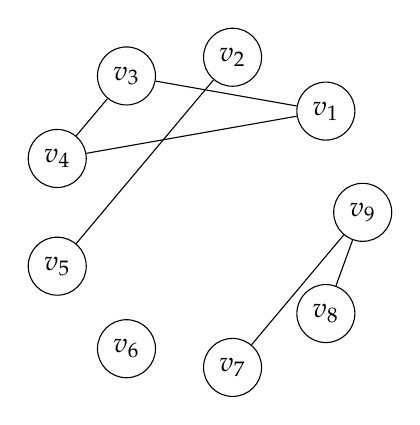
\begin{tikzpicture}
              % Les sommets
              \foreach \i in {1,...,9} {
                \node[circle, draw] (v\i) at (360/9*\i:2) {$v_\i$};
              }

              % Les arêtes
              \draw (v1) -- (v3);
              \draw (v1) -- (v4);
              \draw (v2) -- (v5);
              \draw (v3) -- (v4);
              \draw (v7) -- (v9);
              \draw (v8) -- (v9);
            \end{tikzpicture}
            \end{center}
            \caption{Représentation de la relation $\mathcal{R}$ pour les vecteurs $v_1\to v_9$}
            \end{figure}


            \begin{enumerate}
                \item[2.] Montrer que la relation $\mathcal{R}$ est une relation d'équivalence. Mentionnez explicitement 
                    les techniques de preuves que vous utilisez. 
            \end{enumerate}

            Soit l'ensemble de vecteurs 
            \[ A = \{ (x, y) : x, y \in \mathbb{Z}, x = 0 \leftrightarrow y \neq 0 \}, \] 
            nous devons \textbf{prouver que $\mathcal{R}$ est une relation d'équivalence}.  Pour ce faire, 
            nous allons montrer que $\mathcal{R}$ est réflexive, symétrique et transitive.   

            \begin{prop}{$P_1(v_n, A, \mathcal{R})$}{}
                Tous les vecteurs $v_n$ faisant partie de $A$ respectent la proposition $v_n\mathcal{R}v_n$ : 
                \[ \forall v_n \in A, v_n\mathcal{R}v_n \]
            \end{prop}


            \begin{Preuve}{}{}
                Nous procédons par \textbf{preuve directe}. Supposons que $v_n = (x, y) \in A$. Pour vérfier 
                la réflexivité de $v_n$, nous pouvons appliquer la \textbf{proposition 1.1} sur le vecteur $v_n$. 
                La proposition devient alors $P(x,y, x, y)$ : 
                \[ \Bigl(xy = yx\Bigr) \implies \Bigl(x, y)\mathcal{R}(x,y) \Bigr) \]
                Nous savons que le produit $xy$ est égale à $yx$, par la commutativité de la multiplication. 
                Par l'implication de la proposition 1.1, nous avons alors $(x, y)\mathcal{R}(x, y)$. Ainsi, 
            $v_n\mathcal{R}v_n$ est une proposition vraie et nous concluons alors que $R$ est réflexive. \qed 
            \end{Preuve}


            \begin{prop}{$P_2(v_n, A,\mathcal{R})$}{}
                Tous les vecteurs $v_a = (x, y), v_b = (z, t)$ faisant partie de $A$ sont tels que \textbf{si} 
                $v_a$ est en relation 
                avec $v_b$, \textbf{alors} $v_b$ est en relation avec $v_a$ : 

                \begin{align*}
                    \forall v_a, v_b \in A, v_a &\mathcal{R}v_b  \implies v_b\mathcal{R}v_a  \\ 
                                     &\updownarrow \\ 
                    \forall (x,y),(z, t) \in A, (x, y) &\mathcal{R}(z, t) \implies 
                                     (z, t) \mathcal{R} (x, y)
                \end{align*}
            \end{prop}

            \begin{prop}{}{}
                 Nous procédons pas \textbf{preuve direction}. Supposons que  
                 $(x, y), (z, t) \in A$ et $(x, y)\mathcal{R}(z, t)$. Si $(x, y)\mathcal{R}(x, t)$, alors, 
                 par la définition de la relation $\mathcal{R}$ nous savons que $xt = yz$. 
                 Par l'associativité de la multipliucation, nous savons que 
                 l'équivalence suivante est vraie: 
                 \[ xt = yz \leftrightarrow tx = zy \]
                 \textbf{Or}, $tx = zy$ est simplement $(z, t)\mathcal{R}(x, y)$. En effet, 
                 $(z, t)\mathcal{R}(x, y)$, par la définition de la la relation $\mathcal{R}$, signifie 
                 que $zy = tx$. On sait aussi que, par la réflexitivé de l'égalité, 
                 $a = b \leftrightarrow b = a$. Donc, nous avons : 

                 \begin{align*}
                     (x, y)\mathcal{R}(z, t) \implies xt = yz  & \textbf{\quad Def. de $\mathcal{R}$} \\   
                     xt = yz \implies tx = yz & \textbf{\quad Commutativité de mult.} \\ 
                     tx = yz \leftrightarrow yz = tx & \textbf{\quad Relexivité de l'égalité} \\
                     yz = tx \implies (z, t)\mathcal{R}(x,y) & \textbf{\quad Def. de $\mathcal{R}$ \text{,} inférence}   
                 \end{align*}
            \textbf{Ainsi}, nous avons montré que \textbf{si} $(x, y)\mathcal{R}(z, t)$, \textbf{alors} 
            $(z, t)\mathcal{R}(x, y)$. Nous concluons que $P_2(v_n, A, \mathcal{R})$ est vraie 
            et $\mathcal{R}$ est réflexive. \qed
            \end{prop}

            \begin{prop}{$P_3(x, v_n \mathcal{R}) $}{}
                Tous les vecteurs $v_a = (x, y)$, $v_b = (p, q)$, $v_c = (z, t)$ faisant partie de 
                $A$ sont tels que \textbf{si} $v_a$ est en relation avec $v_b$, et que $v_b$ est en relation avec 
                $v_a$, \textbf{alors}  $v_a$ est en relation avec $v_c$. 
                    \begin{align*}
                        \forall v_a, v_b, v_c \in A, \Bigl(v_a \mathcal{R}v_b\Bigr) &\land  
                    \Bigl(v_b\mathcal{R}v_c\Bigl) \implies \Bigl(v_a \mathcal{R} v_c \Bigr)  \\ 
                                     &\updownarrow \\ 
                    \forall (x,y), (p, q), (z, t) \in A, \Bigl((x, y) &\mathcal{R}(p, q)\Bigr) 
                    \land \Bigl(p, q)\mathcal{R}(z, t)\Bigr) \\ 
                                    &\implies (x, y) \mathcal{R} (z, t)
                    \end{align*}     
            \end{prop}

            \begin{Preuve}{}{}
                Nous procédons par \textbf{preuve directe}. Supposon que 
                $(x,y), (p, q), (z, t) \in A$, que  
                $(x, y) \mathcal{R}(p, q)$ et que  $(p, q)\mathcal{R}(z, t)$
                En supposant que ces deux expressions sont vraie, cela signifie que les deux expressions 
                suivantes sont également vraies : 
                 \begin{align}
                     xq = yp & \textbf{\quad Conséquence de. $v_a\mathcal{R}v_b$} \label{xq = yp}\\ 
                     pt = qz & \textbf{\quad Conséquence de. $v_b\mathcal{R}v_c$} \label{pt = qz}
                 \end{align}

                 \textbf{Or}, en multipliant les deux côtés de l'équation \eqref{xq = yp} par $t$, 
                 et en multipliant les deux côté de l'équation \eqref{pt = qz} par $y$, nous obtenons
                 \begin{align}
                     xqt = ypt \label{xqt = ypt} \\
                     ypt = yqz \label{ypt = yqz}
                 \end{align}

                 Par la transitivité de l'égalité, nous avons : 

                 \begin{align}
                     xqt = yqz \label{xqt = yqz}  
                 \end{align}

                 nous ne pouvons pas diviser les deux côtés de l'équation \eqref{xqt = yqz} par $t$, puisqu'il 
                 est possible que $t$ soit égal à $0$ et que $(z, t) = (z, 0) | z \in \mathbb{Z}, z \neq 0 $. 
                 Mais, à toute fin pratique, nous pouvons ignorer $t$. Si $t$ est égal à zéro, 
                 l'équation \eqref{xqt = yqz} est trivialement vraie ; les deux côté de l'égalité sont égale 
                 à 0. Mais si $t \neq$, nous avons alors l'expression suivante : 
                 \[ xt = yz\]

                 Par la définition de la relation $\mathcal{R}$ nous savons que cette expression signie 
                 $(x, y)\mathcal{R}(z, t)$ ou $v_a\mathcal{R}v_b$. Notons que si $t = 0$, la relation 
                 $(x, y)\mathcal{R}(z, t)$ tient, tant que $y = 0$. Dans ce cas, $(x, y)\mathcal{R}(z, t)$ 
                 découle natuellement de $xqt = yqz$ et toutes les autres équations et dérivations 
                 menant à $(x, y)\mathcal{R}(z, t)$ demeurent vraies. Ainsi, nous avons montré que 
                 \textbf{si}   $(x, y) \mathcal{R}(p, q)$ et que  $(p, q)\mathcal{R}(z, t)$, \textbf{alors}, 
                 $(x, y)\mathcal{R}(z, t)$. Nous concluons donc que $\mathcal{R}$ est transitive. \qed

            \end{Preuve}

            \begin{Reponse*}{}{}
                Nous avons montré que la relation $\mathcal{R}$ est réflexive, symétrique et transitive. 
                Ainsi, nous concluons que $\mathcal{R}$ est, par définition, une relation d'équivalence. \qed 
            \end{Reponse*}



            \section*{Problème 4 $\quad$ $\cdot$  $\quad$ Équivalence des vecteurs}

            \begin{itemize}
                \item Montrez que tout ensemble défini récursivement est dénombrable. Mentionnez explicitement 
                    les techniques de preuves que vous utilisez. 
            \end{itemize}

            \begin{prop}{$P(E, b_i, C_i) $}{}
                 Soit un ensemble $E$ définit récursivement par  
                  \begin{equation*}
                  E = \begin{cases}
                      b_1, b_2, \dots, b_n \Big| \overline{b} = \{b_1, b_2, \dots b_n \} & \text{(\textbf{Bases})},
                        \\
                      C_1, C_2, \dots, C_k \Big| \overline{C} = \{C_1, C_2, \dots C_n \} & \text{(\textbf{Constructeurs})}                    
                        \end{cases}
                \end{equation*}
                Tous les ensemble défini récursivement de cette façon sont dénombrables. 
            \end{prop}

            \begin{Preuve}{}{}
            Nous procédons par \textbf{preuve directe et par induction}. 
            \vspace{1em}\\
            \underline{Hypothèses}
            \vspace{1em}\\
            Soit l'ensemble $E$ définit ci-haut, nous condérons alors les propriétés suivantes : 
            \begin{enumerate}
                \item $b_1, b_2, \dots, b_n$ est un ensemble fini, $\overline{b}$, d'éléments de base définissant 
            l'ensemble $E$ et 
                \item $C_1, C_2, \dots C_k$ est un ensemble fini, $\overline{C}$ de 
            constructeurs manipulant les éléments de base afin de construire de nouveaux éléments 
            appartenant à $E$. 
            \end{enumerate}

            \paragraph{}
            À partir de la définition de $E$, il est alors possible de construir une suite (infinie)
            d'ensembles $E_0, E_1, E_2, \dots$ tels que chaque $E_i$ est une sous-ensemble de $E$. 
            \vspace{1em}\\
            \underline{Constructions d'une suite d'ensembles $E_i$}
            \vspace{1em}\\
            Définissons $E_0$ comme l'ensemble des éléments de base : $E_0 = \overline{b}$. Par l'hypothèse, 
            nous savons que $E_0$ est dénombrable. Définisson également $E_{i+1}$ comme l'ensemble  
            où pour chaque $i \geq 0, E_{i+1}$ est l'ensemble des éléments qui peuvent 
            être construits en utilisant le constructeurs sur $E_i$. Ainsi, pour obtenir $E_1$, par exemple, 
            il faut utiliser tous les constructeurs de $E$ sur tous les éléments de bases de $E_0 = \overline{b}$. 
            \begin{align}
                E_{i+1} \Coloneqq \{ C_j(E_i) \} \label{ C_j(E_i)}                           
            \end{align}
                        

            \underline{Montrer que chaque $E_i$ est dénombrable}
            \vspace{1em}\\
            Par \textbf{l'hypothèse}, $E_0$ est fini et donc dénombrable. Pour construire un premier $E_{i+1}$, soit 
            $E_1$, nous devons nécessairement faire appel à l'appliation de tous les $C_j$ sur $E_0$. 
            Or, nous savons que les $C_j$ sont fini et donc dénombrables et nous savons également que $E_0$ 
            est fini et donc dénombrable. Nous pouvons considérer les constructeurs $C_k$ comme une
            fonction de $E_{i}$ à $E_{i+1}$. 

            \begin{align}
                E_{i+1} = f(C_j, E_i) = \Bigl\{ \sum_{j=1}^{j=k}C_j(E_i) \Bigr\} \label{f(C_j, E_i)}
            \end{align}

            En effet, les $C_j$ donnent les instructions permettant de d'obtenir $E_{i+1}$ à partir 
            de $E_{i}$ et chaque ensemble $\{ C_j(E_i) \}$ est une partition de $E_i$. 
            Nous savons que, à minori, $f(C_j, E_i)$ est surjective, puisqu'il s'agit d'une fonction 
            de $E_i$ à $E_{i+1}$; chaque élément de $E_{i+1}$ peut être mappée sur un seul 
            (si $f(C_j, E_i)$ est injective) ou plusieurs éléments de $E_i$. Puisque $E_i$ est dénombrable 
            et que $f(C_j, E_i)$ est une fonction surjective de $E_i$ à $E_{i+1}$, il s'ensuit que 
            $E_{i+1}$ est dénombre. Notons que $E_{i+1}$, l'image de $f(C_j, E_i)$ peut avoir 
            moins d'éléments que l'ensemble de départ $E_i$, mais ne peut pas en avoir plus. Donc, dans le pire 
            des cas, l'imag eaura la même taille que l'ensemble de départ, ce qui le rend dénombrable et demeure 
            consitant avec la conclusions selon laquelle $E_{i+1}$ est dénombrable. Par ailleurs, 
            nous avons montré, par l'application de la définition de $E$, que 
            $f(C_j, E_i)$ est l'image $E_{i+1}$ de $E_i$. Or, chaque $E_i$ est dénombrable et est une partition 
            de $E$ : 
            \begin{align*}
                E = \bigcup\limits_{i=0}^{\infty}E_i = \bigcup\limits_{i=1}^{i=\infty} \Bigl\{ \sum_{j=1}^{j=k}C_j(E_i) \Bigr\}
            \end{align*}
            Autrement dit, l'union de tous les ensembles $E_i$ obtenus en appliquant tous les constructeurs 
            $C_j$ sur les $E_i$ forment l'ensemble $E$, conformément à la définition récursive de $E$. Puisque 
            chaque $E_i$ est dénombrable, il s'ensuit que l'union $\bigcup\limits_{i=0}^{\infty}E_i$ est également 
            dénombrable. Nous concluons alors que $E$ est dénombrablement infini. Ainsi, tous les 
            ensembles définit récursivement sont dénombrables. \qed 
        

            
           


            \end{Preuve}

            


\end{multicols*}









\end{document}
